% =====================================================================
%  CAPÍTULO 4 -- ESTRATÉGIAS DE IMPLEMENTAÇÃO
%  (Regulamento, Art. 9º, item iv; Art. 10 -- protótipo)
% ---------------------------------------------------------------------
%  Fonte: repositório andreccoelho/roundup_app (branch dev), incluindo
%  docs/decisoes-tecnicas.md e docs/DECISOES_PENDENTES.md.
% =====================================================================

\chapter{Estratégias de implementação}
\label{cap:implementacao}

O protótipo do RoundUp é um aplicativo \textbf{codificado e funcional},
e não apenas um protótipo navegável. Antes da codificação, as telas
principais foram desenhadas como \textit{wireframes} de baixa fidelidade
(17 telas) e organizadas no Figma em três páginas: visão do aluno, visão
do gestor (professor e academia) e cadastro inicial, atendendo ao RNF09.
A implementação aconteceu \textbf{em paralelo} à avaliação das ideias,
entre setembro e novembro de 2026: as ideias do autor foram construídas
como hipóteses desde o início, e os resultados do questionário as
confirmaram, as refutaram ou indicaram ajustes, implementados na etapa de
fechamento (\autoref{sec:rf}). Grande parte do código foi escrita por um
agente de IA, sob o planejamento, o projeto e o controle de qualidade do
autor (\autoref{sec:dev-ia}).

\section{Tecnologias e ferramentas}

O \quadroref{qua:tecnologias} apresenta as tecnologias adotadas e a
justificativa de cada escolha.

\begin{quadrolongo}
\begin{longtable}{|p{3.2cm}|p{4.0cm}|p{6.0cm}|}
  \caption{Tecnologias e ferramentas}\label{qua:tecnologias}\\
  \hline
  \textbf{Finalidade} & \textbf{Tecnologia} & \textbf{Justificativa} \\ \hline
\endfirsthead
  \multicolumn{3}{r}{\textit{(continuação)}}\\
  \hline
  \textbf{Finalidade} & \textbf{Tecnologia} & \textbf{Justificativa} \\ \hline
\endhead
  \multicolumn{3}{r}{\textit{(continua)}}\\
\endfoot
\endlastfoot
    Aplicativo móvel & React Native com Expo (SDK 58) e TypeScript & Base de código única para Android 7.0+, iOS 16.4+ e web (RNF05); tipagem estática reduz erros entre telas e serviços. \\ \hline
    Navegação & React Navigation & Abas e pilhas de telas separadas por perfil. \\ \hline
    Autenticação & Firebase Authentication & Senhas tratadas pelo provedor, sem armazenamento próprio (RNF03). \\ \hline
    Banco de dados & Cloud Firestore & Banco de documentos gerenciado, com regras de segurança declarativas (RNF04). \\ \hline
    Arquivos & Cloud Storage & Fotos de perfil (RF06), com regras próprias. \\ \hline
    Lógica no servidor & Cloud Functions & Tarefas que o cliente não pode fazer com segurança: listas de leitores, público e progresso de missões, registro de medalhas, exclusão de conta e envio de notificações. \\ \hline
    Notificações & Expo Notifications & Registro do aparelho e envio de notificações \textit{push} (RF31). \\ \hline
    Interface & Expo Blur e Expo System UI & Barras translúcidas e acompanhamento do tema claro ou escuro do aparelho. \\ \hline
    Testes & Jest e Firebase Emulator Suite & Testes unitários e testes das regras de segurança e das funções em emulador local. \\ \hline
    Prototipação & Figma & Validação de telas e fluxos antes da codificação (RNF09). \\ \hline
    Modelagem & PlantUML & Diagramas UML versionáveis como texto. \\ \hline
    Gestão do projeto & Notion e Git/GitHub & Base de requisitos e \textit{backlog}; histórico de alterações por ciclo (RNF08). \\ \hline
    Desenvolvimento assistido & Claude Code (agente de codificação da Anthropic), com o \textit{plugin} oficial do Expo & Escrita de código, testes e documentação a partir de requisitos, roteiros e planos do autor, com verificação por testes e regras de segurança (\autoref{sec:dev-ia}). \\ \hline
    Respostas sintéticas & Claude (\texttt{claude-opus-5-5}), Python e Google Apps Script & Apoio à criação das personas e do gerador de respostas; envio das respostas de teste a uma cópia do formulário (\autoref{sec:val-personas}). \\ \hline
\end{longtable}
  \fonte{Elaborado pelo autor (2026).}
\end{quadrolongo}

\section{Arquitetura do aplicativo}

O código foi organizado em camadas. As \textbf{telas}
(\texttt{src/screens}), separadas por perfil (aluno, gestor, academia e
telas compartilhadas), cuidam apenas da apresentação e do estado da
interface. Os \textbf{serviços} (\texttt{src/services}), um por coleção do
banco, concentram o acesso ao Firestore e as transações. As
\textbf{regras de gamificação} ficam em funções puras
(\texttt{src/utils/gamificacao.ts}). Os valores ajustáveis, como pontos
por presença e tabela de níveis, podem ser configurados por cada professor
ou academia (RF33); quando não há configuração, valem os valores-padrão
de \texttt{src/config/gamificacao.ts}. As tarefas que dependem de dados de
vários usuários, como manter as listas de leitores, atualizar o público e o
progresso das missões, registrar medalhas, excluir uma conta em cascata e
enviar notificações, ficam em
\textbf{Cloud Functions} (\texttt{functions/src}). O código-fonte
completo, com as regras de segurança, as suítes de testes e a
documentação das decisões técnicas, está no repositório público
\url{https://github.com/andreccoelho/roundup_app}. A segurança não depende do
aplicativo: as \textbf{regras do Firestore} (\texttt{firestore.rules})
validam cada leitura e escrita no servidor, de modo que um cliente
modificado não consegue, por exemplo, creditar pontos a si mesmo.

As telas de professor e de academia compartilham a mesma estrutura de
navegação de ``gestor'' (turmas, alunos e missões), e a academia recebe
abas adicionais para gerenciar professores e consultar a visão
consolidada. Isso reproduz no código a generalização entre os atores
descrita no \autoref{cap:modelagem}.

\section{Etapas de desenvolvimento}

O desenvolvimento seguiu os quatro ciclos definidos nos requisitos, do
núcleo para os recursos complementares, e foi intercalado com a avaliação
das ideias. O \quadroref{qua:linha-tempo} mostra a sequência real das
etapas, reconstruída a partir do histórico do repositório.

\begin{quadrolongo}
\begin{longtable}{|p{3.0cm}|p{10.3cm}|}
  \caption{Linha do tempo do projeto}\label{qua:linha-tempo}\\
  \hline
  \textbf{Data (2026)} & \textbf{Etapa} \\ \hline
\endfirsthead
  \multicolumn{2}{r}{\textit{(continuação)}}\\
  \hline
  \textbf{Data (2026)} & \textbf{Etapa} \\ \hline
\endhead
  \multicolumn{2}{r}{\textit{(continua)}}\\
\endfoot
\endlastfoot
    1 a 10 set. & Ciclo 1 -- base: cadastro e autenticação dos três perfis, vínculos, turmas, matrículas, sessões, \textit{check-in} com janela de tempo, agenda e histórico (RF01 a RF08, RF10 a RF15), regras de segurança e primeira suíte de testes em emulador. Lista de requisitos versionada em 8 set. \\ \hline
    8 a 15 set. & Ciclos 2 a 4 -- primeira versão de gamificação (RF16 a RF21), gestão (RF09, RF22 a RF27), conformidade e retenção (RF28 a RF32, incluindo preferências de notificação por tipo) e primeira rodada de ajustes de interface. \\ \hline
    18 e 19 set. & Questionário com usuários reais: confirmação ou refutação das ideias (\autoref{sec:val-survey}). \\ \hline
    15 out. & Segunda rodada de interface (\textit{redesign} ``Noite de luta''). \\ \hline
    26 out. & Personas e respostas sintéticas: ideias novas, sinal complementar e teste do questionário (\autoref{sec:val-personas}). \\ \hline
    5 a 12 nov. & Fechamento: classificação mensal com adesão opcional, exclusão de conta em cascata, progresso das missões, personalização da pontuação, envio de notificações, sequência contada por sessões, dados pessoais em documento privado (RNF04), política de privacidade definitiva (RF28), graduação por modalidade (RF06, RF25, RN03), edição e exclusão de turmas (RF10, RF12) e encerramento de vínculos e saída de turmas (RF07, RF08, RF11). Terceira rodada de interface, segundo as diretrizes da Apple. \\ \hline
    13 nov. & Conclusão dos requisitos parciais: medalhas com data de conquista (RF19), público e vigência das missões (RF23), estrutura de faixas por modalidade com barra de progresso (RF33 e RF25), teste de notificações em aparelho (RF31) e atualização do Expo SDK de 57 para 58. Execução em iPhone, correção dos defeitos encontrados (\autoref{sec:defeitos-testes}) e execução final das suítes de teste. \\ \hline
\end{longtable}
  \fonte{Elaborado pelo autor (2026), a partir do histórico de \textit{commits} do repositório.}
\end{quadrolongo}

A primeira versão de todos os ciclos ficou pronta antes do questionário,
o que é próprio do processo de ideação adotado: o aplicativo funcionou
como a materialização das hipóteses do autor, e a avaliação definiu o que
seria mantido, ajustado ou revisto nas etapas seguintes. As três rodadas
de interface terminaram seguindo as diretrizes de interface da Apple
(\textit{Human Interface Guidelines}), com temas claro e escuro que
acompanham o aparelho, fonte e escala tipográfica do sistema, listas
agrupadas, barras translúcidas e anel de progresso, preservando a marca, o
vermelho de destaque e um fundo discreto de lona de ringue nos cartões
principais.

A \autoref{fig:telas} mostra seis telas do protótipo na versão final
da interface.

\begin{figure}[H]
  \centering
  \caption{Telas do protótipo: (a) acesso; (b) início do aluno; (c) classificação; (d) perfil do aluno; (e) missões; (f) chamada do professor}
  \label{fig:telas}
  \setlength{\fboxsep}{0pt}\setlength{\fboxrule}{0.3pt}
  \begin{tabular}{ccc}
    \fbox{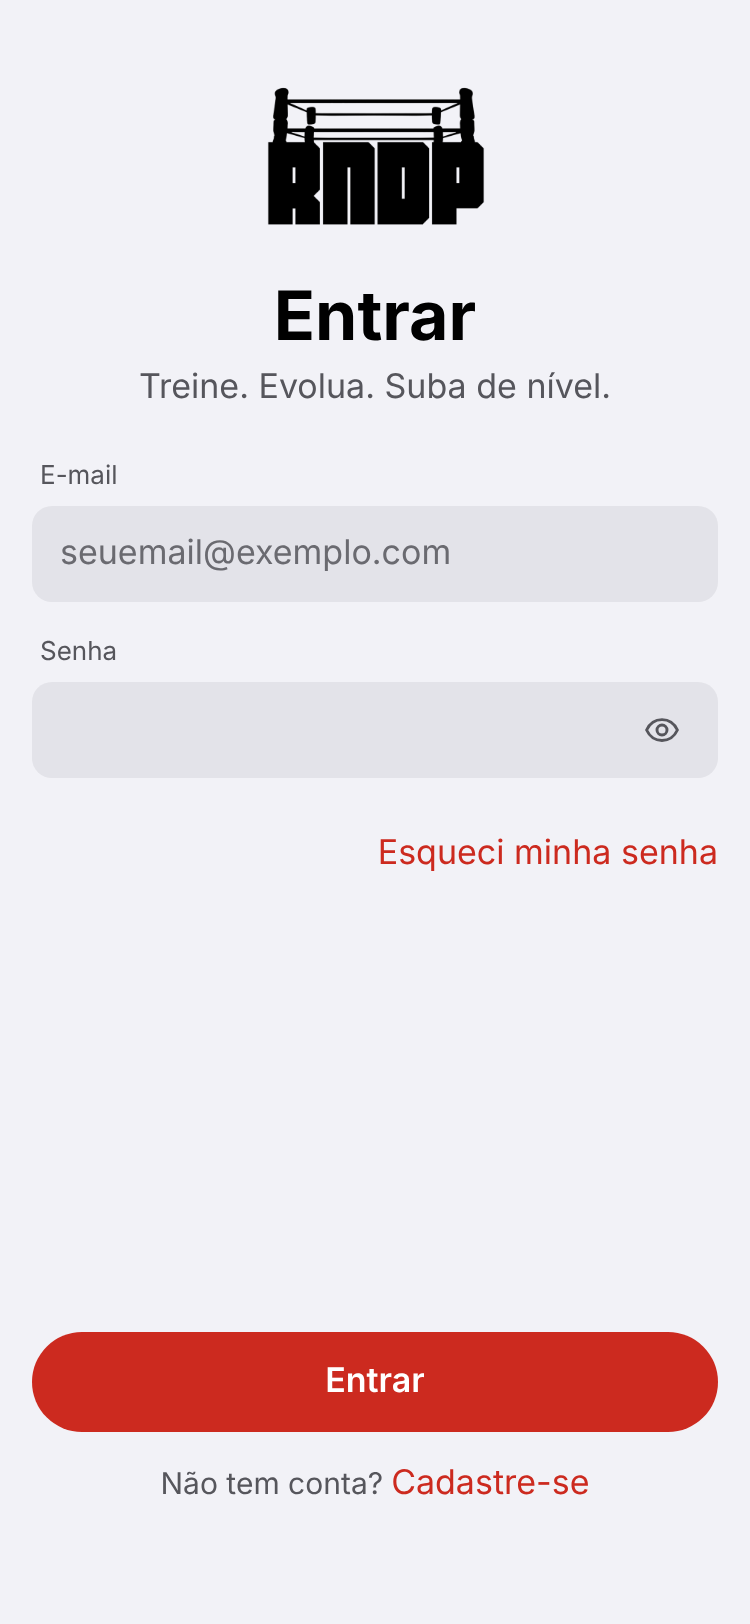
\includegraphics[width=0.27\textwidth]{figuras/tela-login.png}} &
    \fbox{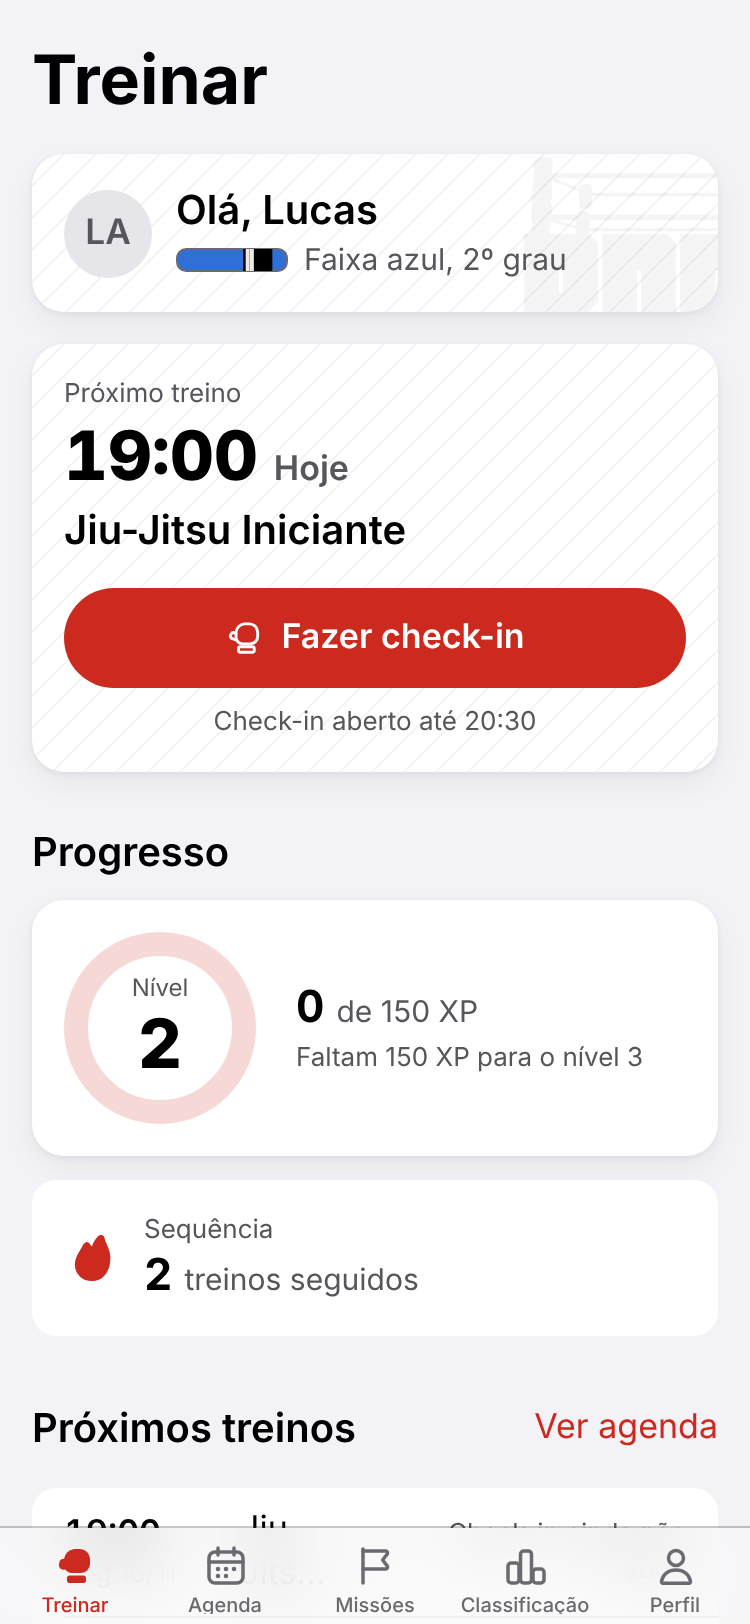
\includegraphics[width=0.27\textwidth]{figuras/tela-aluno-inicio.png}} &
    \fbox{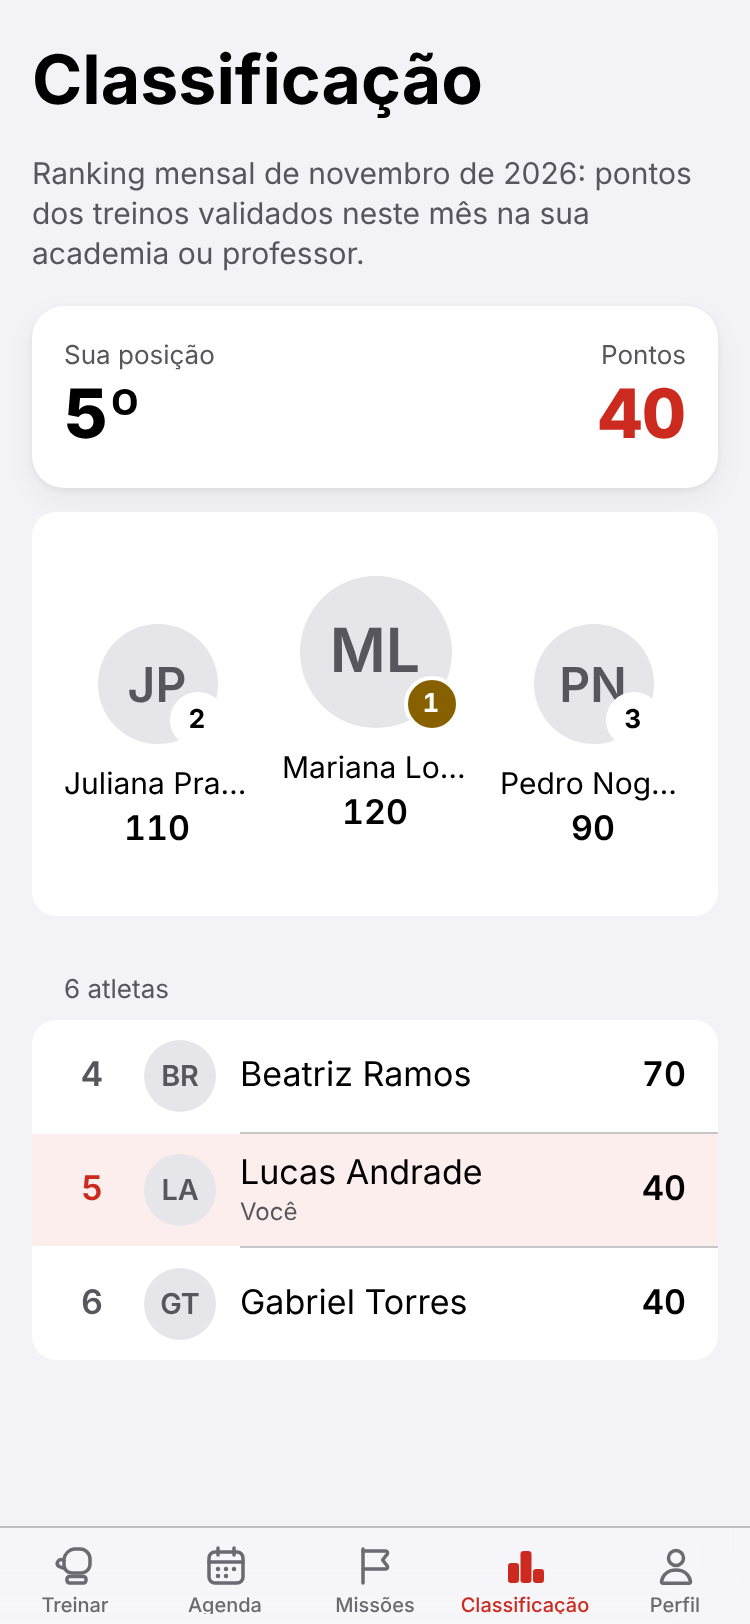
\includegraphics[width=0.27\textwidth]{figuras/tela-aluno-classificacao.png}} \\
    \footnotesize (a) & \footnotesize (b) & \footnotesize (c) \\[6pt]
    \fbox{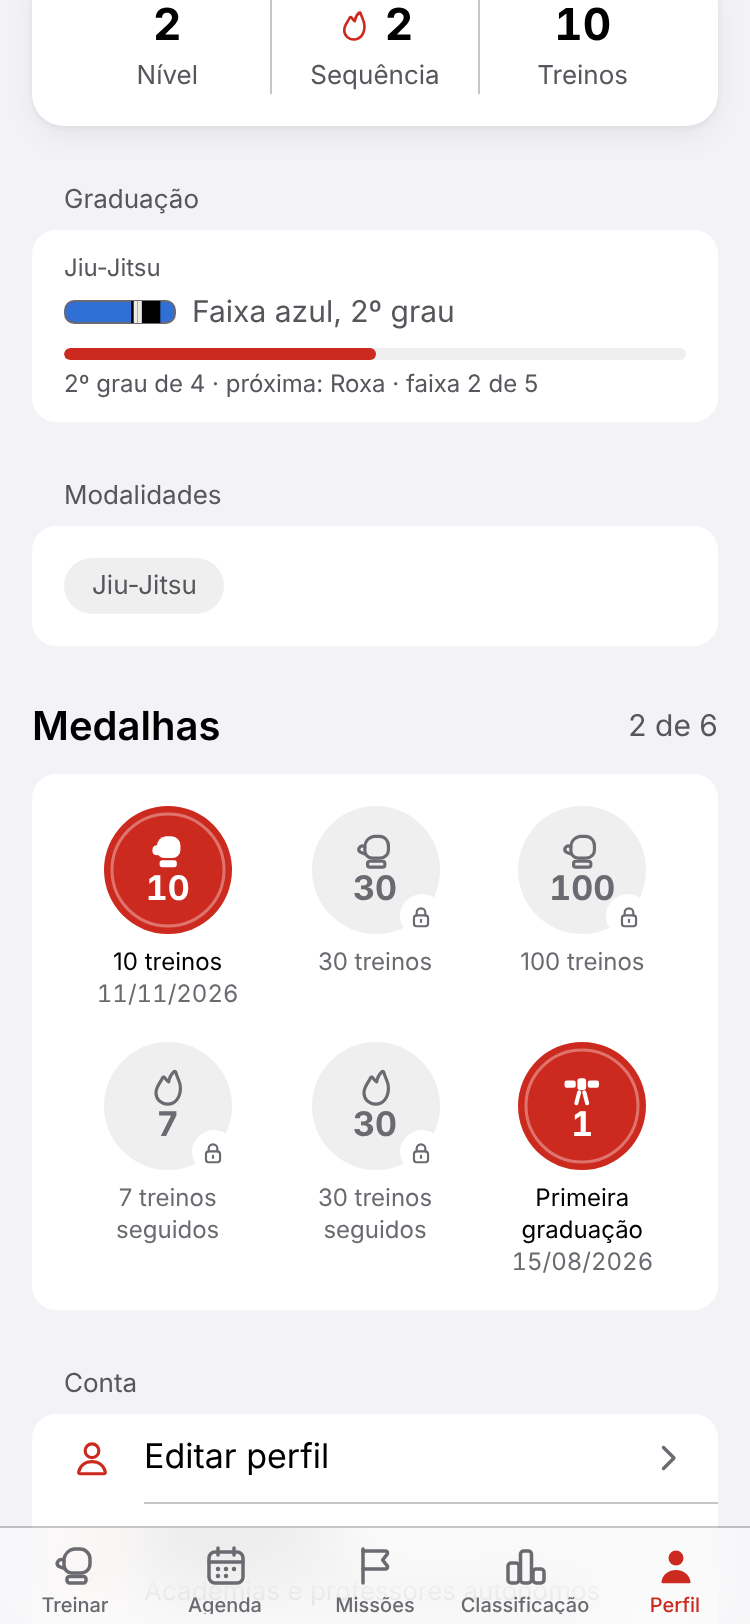
\includegraphics[width=0.27\textwidth]{figuras/tela-aluno-perfil.png}} &
    \fbox{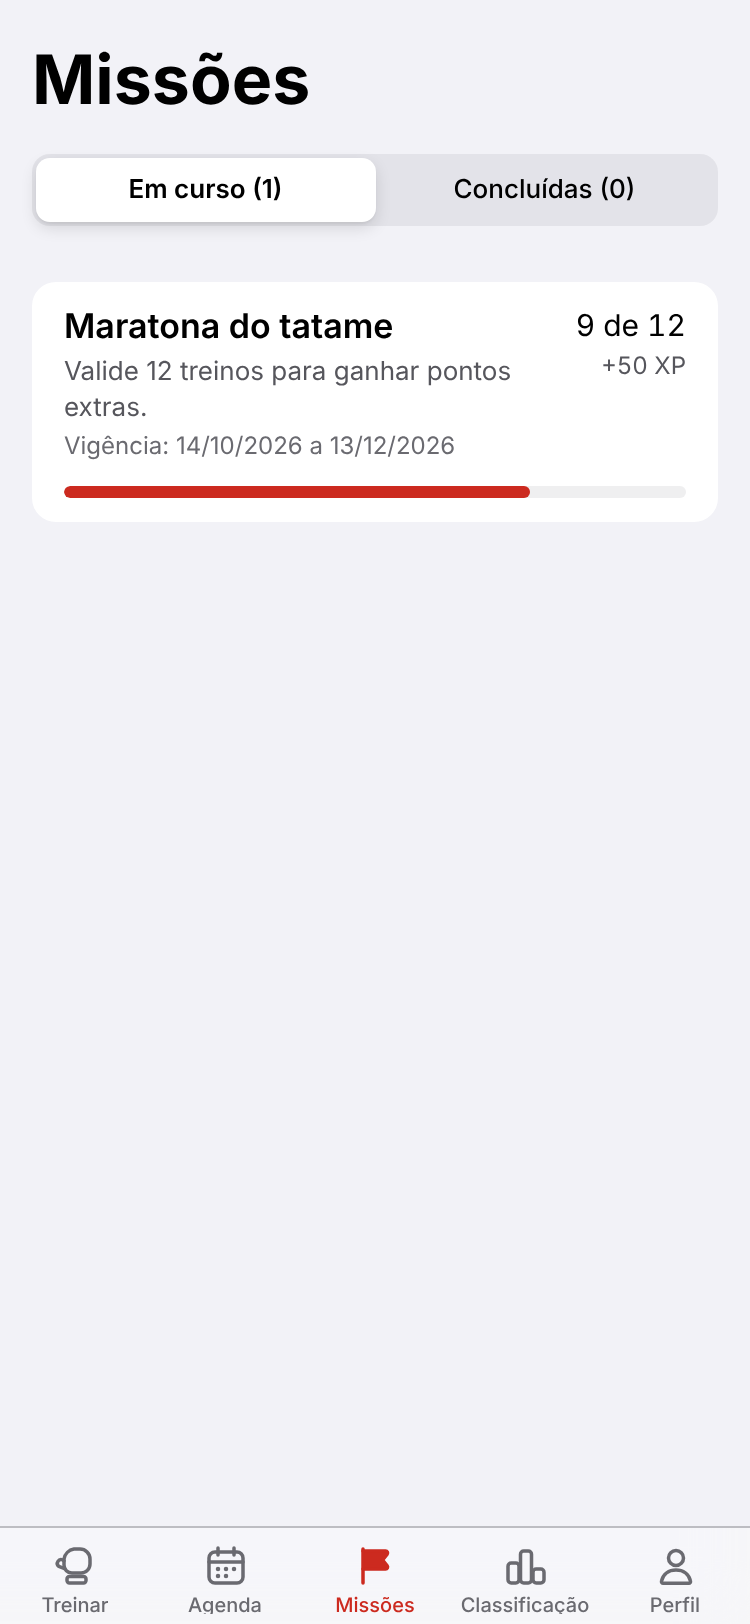
\includegraphics[width=0.27\textwidth]{figuras/tela-aluno-missoes.png}} &
    \fbox{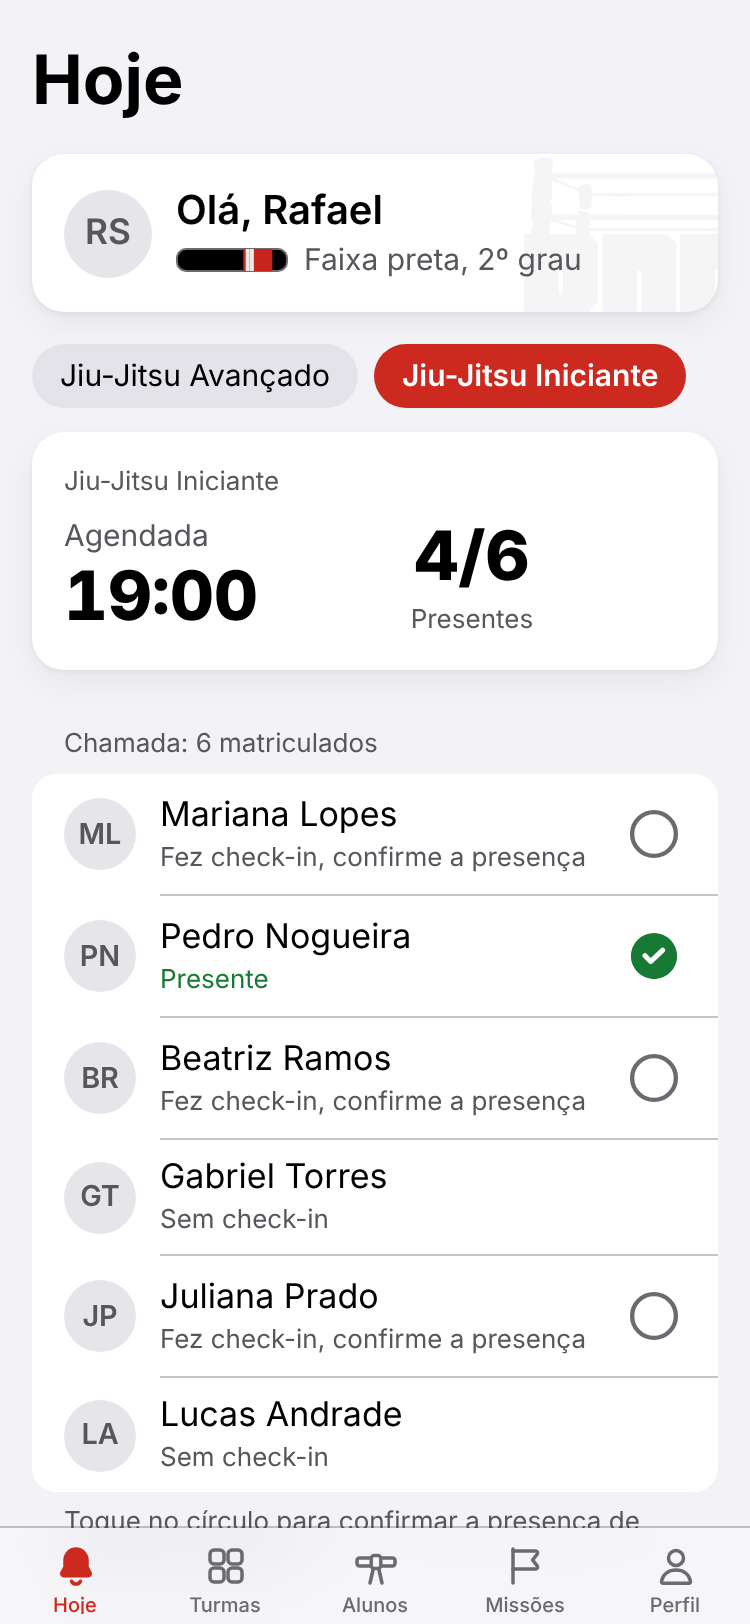
\includegraphics[width=0.27\textwidth]{figuras/tela-professor-chamada.png}} \\
    \footnotesize (d) & \footnotesize (e) & \footnotesize (f)
  \end{tabular}
  \fonte{Elaborado pelo autor (2026). Tema claro; as telas (b) a (f) foram
         capturadas na versão web, com dados fictícios.}
\end{figure}

Na tela inicial do aluno (b), o cartão do próximo treino traz o botão de
\textit{check-in} a um toque de distância, o que atende ao RNF01; logo
abaixo aparecem o anel de progresso, com o nível e o XP que falta para o
próximo, e a sequência de treinos. Na classificação (c), o aluno vê a sua
posição no mês e a linha dele aparece destacada. No perfil (d), a barra
de graduação mostra o grau atual dentro da faixa e a próxima faixa da
estrutura do responsável (RF33), e as medalhas conquistadas exibem a data
da conquista (RF19). Nas missões (e), cada missão mostra o progresso, a
recompensa e o período de vigência (RF23). Na chamada do professor (f),
cada aluno que fez \textit{check-in} tem a presença confirmada com um
toque no círculo.

\section{Desenvolvimento assistido por agentes de IA}
\label{sec:dev-ia}

Como discutido no \autoref{cap:introducao}, o uso de IA já é a regra no
desenvolvimento de software \cite{dora2025,stackoverflow2025}, mas seus
ganhos dependem de como ela é usada: práticas como controle de versão,
revisão e padrões de desenvolvimento continuam sendo a base que permite
aproveitá-la \cite{dora2025}, e o trabalho do desenvolvedor experiente
pode até ficar mais lento quando o código gerado exige muita revisão
\cite{becker2025}. Neste projeto, a maior parte do código foi escrita por
um agente de codificação (Claude Code), e o autor concentrou o seu papel
nas atividades que o agente não substitui: planejar, projetar e controlar
a qualidade. O \quadroref{qua:papeis} resume essa divisão, conforme
registrada no repositório.

\begin{quadrolongo}
\begin{longtable}{|>{\raggedright\arraybackslash}p{2.8cm}|>{\raggedright\arraybackslash}p{5.6cm}|>{\raggedright\arraybackslash}p{4.9cm}|}
  \caption{Divisão de papéis entre o autor e o agente de IA}\label{qua:papeis}\\
  \hline
  \textbf{Atividade} & \textbf{Autor} & \textbf{Agente de IA} \\ \hline
\endfirsthead
  \multicolumn{3}{r}{\textit{(continuação)}}\\
  \hline
  \textbf{Atividade} & \textbf{Autor} & \textbf{Agente de IA} \\ \hline
\endhead
  \multicolumn{3}{r}{\textit{(continua)}}\\
\endfoot
\endlastfoot
    Planejamento & Ideias, requisitos, prioridades e ciclos; roteiros de cada tarefa, com critérios de aceite e restrições & Lê os roteiros e o estado do código antes de agir \\ \hline
    Projeto & Modelo de atores, modelo de dados, regras de negócio e decisões de arquitetura; decisão sobre conflitos e dependências novas & Propõe planos, aponta conflitos e limitações técnicas encontradas \\ \hline
    Implementação & Revisão e aceite de cada etapa & Escreve código, testes e registros de decisões, uma etapa por \textit{commit} \\ \hline
    Controle de qualidade & Critérios de teste, execução das suítes, regras de segurança no servidor, execução em aparelho e aceite final & Corrige os defeitos apontados pelos testes e pela execução \\ \hline
\end{longtable}
  \fonte{Elaborado pelo autor (2026).}
\end{quadrolongo}

Quatro mecanismos, todos registrados no repositório, mantiveram o agente
sob controle:

\begin{enumerate}
  \item \textbf{Instruções permanentes no repositório.} Os arquivos
        \texttt{CLAUDE.md} e \texttt{AGENTS.md}, lidos pelo agente a cada
        sessão, apontam a lista oficial de requisitos, exigem os códigos
        dos requisitos nos comentários de rastreabilidade e obrigam a
        consulta à documentação da versão exata do Expo SDK, o que evita
        o uso de interfaces de versões anteriores.
  \item \textbf{Roteiro, auditoria e plano antes do código.} Cada tarefa
        maior partiu de um roteiro escrito pelo autor, com critérios de
        aceite e restrições, como a de não instalar dependências sem
        aprovação. Antes de codificar, o agente produzia uma auditoria ou
        um plano. Na auditoria da interface, por exemplo, ele encontrou
        três conflitos entre o roteiro e a especificação visual em vigor e
        os devolveu ao autor, em vez de resolvê-los sozinho; no plano das
        regras de segurança dos Ciclos 2 e 3, mostrou que duas das quatro
        telas pedidas não precisavam de regra nova e que a classificação
        ainda não tinha estrutura de dados, o que exigiu projetá-la
        antes de escrever as suas regras.
  \item \textbf{Pequenos lotes.} As mudanças foram feitas em etapas
        curtas, uma por \textit{commit} (o \textit{redesign} de interface,
        por exemplo, foi dividido em oito fases), o que torna cada
        mudança revisável e reversível. Entre 1º de setembro e 15 de
        novembro, o repositório recebeu 129 \textit{commits}, concentrados
        em 12 dias de trabalho, e chegou a cerca de 18 mil linhas de
        TypeScript e 679 linhas de regras de segurança.
  \item \textbf{Verificação independente do agente.} A segurança não
        depende de o código gerado estar certo: as regras do Firestore
        validam cada operação no servidor, e as suítes automatizadas
        (\autoref{sec:testes-prototipo}) verificam o comportamento
        esperado em emulador. Os testes refutaram hipóteses técnicas
        adotadas durante o desenvolvimento, como a de que o Firestore
        reaproveitaria leituras entre documentos de uma mesma consulta, e
        revelaram defeitos que só a execução mostrou
        (\autoref{sec:defeitos-testes}).
\end{enumerate}

Esse arranjo tem limites que devem ser explicitados. O histórico do
repositório não distingue o que foi escrito pelo agente do que foi
escrito ou alterado pelo autor, e o projeto não teve uma condição de
comparação sem IA; por isso, este relatório não mede ganho de
produtividade, apenas descreve o processo e os controles adotados. A
responsabilidade pelo resultado permanece do autor, que aprovou cada
etapa e verificou o produto final.

\section{Situação de implementação dos requisitos}
\label{sec:situacao-implementacao}

O \quadroref{qua:implementacao} resume o que foi implementado. As
limitações remanescentes foram registradas no repositório como decisões
pendentes, para que fiquem explícitas, e não escondidas na interface. O
critério de compatibilidade do RNF05 foi revisado de iOS 14 para iOS
16.4, versão mínima exigida pelo Expo SDK 58, adotado na etapa final; no
Android, o mínimo do SDK (Android 7.0) já atende ao critério original.

\begin{quadrolongo}
\begin{longtable}{|p{2.2cm}|p{4.2cm}|p{7.0cm}|}
  \caption{Situação de implementação dos requisitos}\label{qua:implementacao}\\
  \hline
  \textbf{Situação} & \textbf{Requisitos} & \textbf{Observação} \\ \hline
\endfirsthead
  \multicolumn{3}{r}{\textit{(continuação)}}\\
  \hline
  \textbf{Situação} & \textbf{Requisitos} & \textbf{Observação} \\ \hline
\endhead
  \multicolumn{3}{r}{\textit{(continua)}}\\
\endfoot
\endlastfoot
    Implementado & RF01--RF33; RN01--RN09; RNF01--RNF05, RNF07--RNF11 & Funcionalidades disponíveis nas telas e cobertas, na parte de segurança e de servidor, por testes em emulador. A interface foi conferida na versão web, e RF19, RF23, RF31 e RF33 também foram verificados em um iPhone. O tempo de carregamento (RNF02) foi medido na tela inicial, em 4G (\autoref{sec:testes-prototipo}). No Android, a compatibilidade (RNF05) decorre da versão mínima do SDK, sem execução em aparelho registrada. \\ \hline
    Não implementado & RNF06 & Decisão de projeto: o \textit{check-in} e a validação de presença são gravados em transações que exigem conexão, porque o servidor precisa garantir a janela de horário (RN08) e o limite de um \textit{check-in} por sessão (RN02). Um registro feito sem conexão poderia ser recusado depois, quando o aluno já acreditasse ter treinado com pontos garantidos. \\ \hline
\end{longtable}
  \fonte{Elaborado pelo autor (2026), a partir do repositório do projeto.}
\end{quadrolongo}

Os valores de gamificação têm um padrão, usado quando o professor ou a
academia não configuram os seus: 10 pontos por presença validada, dez
níveis com limiares crescentes (100, 250, 450\ldots{} até 3.250 pontos) e
medalhas para 10, 30 e 100 treinos, para sequências de 7 e 30 sessões e
para a primeira graduação. Esses valores permitiram construir e testar a
interface, mas ainda precisam ser calibrados com uso real.

Na conclusão dos requisitos que estavam parciais, quatro decisões
merecem registro:

\begin{itemize}
  \item \textbf{Medalhas (RF19).} Cada medalha é gravada em
        \texttt{usuarios/\{aluno\}/medalhas}, com a data de conquista,
        somente por Cloud Function; o aplicativo não consegue escrevê-la.
        O estorno de um \textit{check-in} não retira uma medalha já
        conquistada, e um \textit{script} de migração reconstruiu, a partir
        do histórico, a data das medalhas dos alunos existentes.
  \item \textbf{Missões (RF23).} O gestor define o público (todos os alunos
        vinculados, uma turma ou alunos escolhidos) e a vigência. A regra
        vale no banco de dados, não só na tela: só o público lê a missão,
        a conclusão manual só é aceita dentro da vigência, o progresso
        automático só conta treinos do período e o aviso de nova missão
        (RF31) vai só para o público, uma vez por aluno. Depois do fim da
        vigência, a missão continua no histórico de quem a concluiu.
  \item \textbf{Faixas (RF33).} O gestor personaliza, por modalidade, a
        ordem, o nome, a cor e o número de graus de cada faixa; sem
        personalização, vale a lista anterior como padrão. O registro de
        graduação (RF25) passou a gravar a faixa de forma estruturada, e o
        perfil do aluno ganhou a barra de progresso até a próxima
        graduação, medida pelos graus da faixa atual (por exemplo, ``2º
        grau de 4 · próxima: Roxa''). Graduações antigas, registradas como
        texto livre, foram convertidas por um \textit{script} que reconhece
        o nome da faixa; os textos sem correspondência permanecem como
        texto.
  \item \textbf{Notificações (RF31).} O projeto foi preparado para gerar
        versões instaláveis pelo EAS, e a tela de preferências de
        notificação ganhou botões para enviar uma notificação de teste ao
        próprio aparelho, o que permitiu validar o envio em um iPhone.
\end{itemize}

\section{Detalhes de implementação}

\subsection{Crédito de pontos com validação humana}

O \autoref{cod:validar} mostra o núcleo da função que confirma uma
presença. A confirmação e o crédito acontecem em uma única transação: o
\textit{check-in} recebe os pontos configurados pelo responsável e a
classificação do aluno, no escopo daquele responsável e no mês da sessão,
é atualizada. Se o professor desfizer a confirmação, os pontos são
estornados. A regra de segurança confere o \textit{check-in} e a
classificação na mesma transação: o crédito só pode ser o valor
configurado, e o estorno só pode devolver o que o \textit{check-in}
recebeu. Isso impede créditos arbitrários mesmo que alguém altere o
aplicativo.

\begin{codigo}[H]
  \caption{Validação de presença e crédito de pontos (TypeScript, trecho)}
  \label{cod:validar}
\begin{lstlisting}
await runTransaction(db, async (transacao) => {
  const checkin = (await transacao.get(checkinRef)).data() as CheckIn;
  const vaiCreditar = novoStatus === 'validado' && checkin.pontos === 0;
  const vaiEstornar = novoStatus === 'pendente' && checkin.pontos > 0;
  const periodo = periodoDe(checkin.dataHora.toDate());          // AAAA-MM
  const classificacaoId = vaiEstornar && checkin.classificacaoId
    ? checkin.classificacaoId
    : `${checkin.alunoId}_${checkin.responsavelId}_${periodo}`;
  const classificacaoRef = doc(db, 'classificacoes', classificacaoId);
  let pontosAtuais = 0, pontosDoCheckin = 0;
  if (vaiCreditar || vaiEstornar) {
    const snap = await transacao.get(classificacaoRef);
    pontosAtuais = snap.exists() ? snap.data().pontos : 0;
  }
  if (vaiCreditar) {                    // valor configurado ou padrao (RF33)
    const config = await transacao.get(doc(db, 'configuracoesGamificacao',
                                           checkin.responsavelId));
    pontosDoCheckin = config.exists() ? config.data().pontosPorCheckin
                                      : XP_POR_CHECKIN_VALIDADO;
  }
  transacao.update(checkinRef, {
    status: novoStatus, validadoPor: responsavelId,
    pontos: vaiCreditar ? pontosDoCheckin : vaiEstornar ? 0 : checkin.pontos,
    ...(vaiCreditar || vaiEstornar ? { classificacaoId } : {}),
  });
  if (vaiCreditar || vaiEstornar) {
    const delta = vaiCreditar ? pontosDoCheckin : -checkin.pontos;
    transacao.set(classificacaoRef, { pontos: pontosAtuais + delta,
      periodo: classificacaoId.slice(-7), origemCheckinId: checkinId },
      { merge: true });
  }
});
\end{lstlisting}

  \fonte{Elaborado pelo autor (2026), adaptado de \texttt{src/services/checkins.ts}.}
\end{codigo}

\subsection{Cálculo da sequência de treinos}

A sequência (RF21) conta as \textbf{sessões consecutivas} das turmas do
aluno em que ele teve presença validada, da mais recente para a mais
antiga (\autoref{cod:sequencia}). Sessões canceladas não contam, e uma
sessão com a janela de \textit{check-in} ainda aberta, ou com
\textit{check-in} aguardando validação, é ignorada, para não interromper a
sequência antes da hora. Assim, um dia sem aula não quebra a sequência:
ela só é interrompida quando houve sessão e o aluno não compareceu. O
mesmo critério é usado no aplicativo e nas Cloud Functions que avaliam as
missões de sequência.

\begin{codigo}[H]
  \caption{Cálculo da sequência de treinos por sessão (TypeScript)}
  \label{cod:sequencia}
\begin{lstlisting}
export function calcularSequencia(sessoes: Sessao[], checkins: CheckIn[],
                                  agora: Date = new Date()): number {
  const statusPorSessao = new Map(checkins.map((c) => [c.sessaoId, c.status]));
  const maisRecentesPrimeiro = sessoes
    .filter((s) => s.status !== 'cancelada')
    .sort((a, b) => b.janelaCheckInFim.toMillis() - a.janelaCheckInFim.toMillis());
  let sequencia = 0;
  for (const sessao of maisRecentesPrimeiro) {
    const status = statusPorSessao.get(sessao.id);
    if (status === 'validado') sequencia += 1;
    else if (sessao.janelaCheckInFim.toDate() > agora || status === 'pendente') continue;
    else break;                         // houve sessao e o aluno nao foi
  }
  return sequencia;
}
\end{lstlisting}
  \fonte{Elaborado pelo autor (2026), adaptado de \texttt{src/utils/gamificacao.ts}.}
\end{codigo}